%% RC-Gate -- Springer Nature (sn-jnl), single-column layout
\documentclass[pdflatex,sn-mathphys,Numbered]{sn-jnl}

\usepackage{graphicx}%
\usepackage{multirow}%
\usepackage{amsmath,amssymb,amsfonts}%
\usepackage{amsthm}%
\usepackage{mathrsfs}%
\usepackage{xcolor}%
\usepackage{textcomp}%
\usepackage{manyfoot}%
\usepackage{booktabs}%
\usepackage{algorithm}%
\usepackage{algorithmicx}%
\usepackage{algpseudocode}%
\usepackage{array}%
\usepackage{tikz}%
\usetikzlibrary{arrows.meta,positioning,shapes.geometric,fit,backgrounds}%

\raggedbottom

\begin{document}

\title[RC-Gate for black-box hallucination detection]{RC-Gate: A Reliability-Conditioned Gated Mixture-of-Experts for Black-Box Hallucination Detection, with Controlled and Real-Data Evaluation}

\author[1]{\fnm{P. T.} \sur{Rangesh Pandian}}
\email{rangeshpandian@gmail.com}

\author[1]{\fnm{G.} \sur{Vishal}}
\email{vishalgastu30@gmail.com}

\author*[1]{\fnm{Divya} \sur{Mohan}\textsuperscript{[0000-0002-5988-3851]}}
\email{divyamohan797@gmail.com}

\affil*[1]{
\orgdiv{Department of Computing Technologies},
\orgname{SRM Institute of Science and Technology},
\orgaddress{\city{Kattankulathur}, \postcode{603203}, \state{Tamil Nadu}, \country{India}}
}

\abstract{Black-box hallucination detectors for large language models routinely combine two noisy, partially complementary signal families: cross-model consensus and retrieval-based evidence grounding. Existing hybrid detectors integrate these families using a single global rule, such as static scalar blending or monolithic feature concatenation, which implicitly assumes that signal reliability remains uniform across diverse operational contexts. We investigate whether dynamically conditioning this combination on lightweight, non-invasive metadata available at inference time improves claim-level hallucination detection. We present RC-Gate (Reliability-Conditioned Gate), a lightweight mixture-of-experts architecture containing 229 trainable parameters in our synthetic deployment that conditions exclusively on claim type and generator identity. RC-Gate routes claims to specialist linear experts via a temperature-scaled softmax gate and fuses their outputs at the logit level, returning calibrated routing weights alongside an uncalibrated hallucination risk score to provide transparent, glass-box attribution. We evaluate RC-Gate on controlled synthetic signal tables with planted statistical dependencies (13,500 claims across five seeds) and on the real-world RAGTruth benchmark (800 claims across six language models and three seeds). In controlled experiments, RC-Gate validates its architectural machinery by outperforming flat logistic fusion by $+0.118$ AUROC overall and $+0.377$ on numeric claims, recovering 0.748 AUROC on an unseen inverted generator where flat fusion collapses to 0.171. However, two rigorous controls qualify this success: an unconstrained gradient-boosted tree baseline supplied with identical metadata outperforms RC-Gate (0.929 vs.\ 0.874 AUROC), and conditioning on claim type alone accounts for virtually all gating utility. On RAGTruth, RC-Gate fails to outperform flat baselines (0.631 vs.\ 0.681 for flat logistic regression and 0.740 for gradient boosting), with paired bootstrap intervals spanning zero ($-0.050$ [$-0.210, 0.100$]) and routing weights collapsing toward uniformity. We document this real-data negative result transparently, provide an empirical post-mortem of the domain transfer gap, and outline five constructive, concrete future-work programs for conditional hallucination detection.}

\keywords{hallucination detection, mixture of experts, gated fusion, black-box verification, cross-model consistency, retrieval-augmented generation, negative results}

\maketitle

%% ====================================================================
\section{Introduction}\label{sec:intro}
%% ====================================================================

Large language models (LLMs) frequently generate syntactically fluent assertions that contradict reference materials or assert ungrounded falsehoods, often delivered with identical linguistic confidence as verified truths~\cite{ji2023survey}. Detecting such hallucinations without white-box access to model weights or internal hidden activations (the \emph{black-box} regime) is of immense practical significance, as commercial deployments predominantly consume LLMs via closed proprietary APIs. In this regime, two primary signal paradigms have emerged:
\begin{enumerate}
    \item \textbf{Cross-Model Consensus Signals}: Methods that evaluate whether independent generator instances corroborate or contradict an asserted claim, either via stochastic self-resampling~\cite{manakul2023selfcheckgpt} or through heterogeneous multi-model panels~\cite{chen2024beacon}.
    \item \textbf{Evidence-Grounded Verification Signals}: Methods that decompose responses into atomic factual statements and verify each statement against retrieved reference documents using Natural Language Inference (NLI) cross-encoders~\cite{min2023factscore,dhuliawala2023chain}.
\end{enumerate}

Neither signal family provides universal reliability. Cross-model consensus suffers catastrophic failure when multiple language models share common inductive biases, pre-training corpora, or common misconceptions, leading to unanimous but entirely false agreement. Conversely, evidence grounding fails when retrieval indices return incomplete contexts, when documents contain internal contradictions, or when assertions require multi-hop arithmetic computation rather than lexical lookup.

To mitigate these localized vulnerabilities, contemporary systems combine both paradigms into hybrid detectors. However, virtually all published hybrid architectures enforce a \emph{monolithic global rule}, such as static scalar blending ($\alpha \cdot s_{\mathrm{cross}} + (1-\alpha) \cdot s_{\mathrm{evid}}$)~\cite{ding2024rowen} or flat feature pooling into a single classifier~\cite{zhao2024medico}. A global rule cannot express context-dependent routing policies, such as: \emph{``Heavily weight evidence grounding for arithmetic and numeric assertions; weight multi-model consensus for named entity assertions; and explicitly distrust the consensus signal when evaluating a known, poorly-calibrated generator.''}

In this paper, we introduce and systematically evaluate \textbf{RC-Gate} (Reliability-Conditioned Gate), a lightweight, metadata-only gated Mixture-of-Experts (MoE) for claim-level hallucination detection. RC-Gate maintains a strict \emph{metadata isolation barrier}: the gating network observes only lightweight contextual metadata—specifically the linguistic claim type $t$ and generator identity $g$—without observing the raw verification signals themselves. The gate outputs dynamic trust weights $(w_{\mathrm{cross}}, w_{\mathrm{evid}})$ that modulate specialist linear experts scoring the claim from their respective feature representations. The experts are fused at the logit level via a stacked meta-learner~\cite{wolpert1992stacked}, returning an uncalibrated hallucination risk score alongside the trust weights to deliver interpretable, glass-box diagnostic explanations.

We formulate three formal research hypotheses:
\begin{itemize}
    \item \textbf{H1 (Conditional Signal Reliability)}: The empirical diagnostic value of cross-model consensus and evidence grounding varies systematically across claim types and generator identities.
    \item \textbf{H2 (Gated Routing Superiority)}: A reliability-conditioned gating network outperforms flat linear fusion and static blending, exhibiting its greatest margin on numeric and extractive assertions.
    \item \textbf{H3 (Weight Interpretability)}: The learned gate weights faithfully recover the underlying reliability regimes, assigning near-zero weight to unreliable signal families in domains where their failure is planted or documented.
\end{itemize}

Crucially, the core contribution of this work lies as much in its rigorous experimental evaluation and negative findings as in its architectural proposal. Specifically, our contributions are:
\begin{enumerate}
    \item We design RC-Gate, a 229-parameter metadata-isolated gated mixture-of-experts for claim-level hallucination detection, featuring logit-level expert fusion and transparent natural-language attribution.
    \item We construct a synthetic benchmark with planted conditional reliability (13,500 claims across five seeds) to mathematically validate the gating machinery, alongside a leave-one-generator-out (LOGO) cold-start evaluation on an unseen inverted generator.
    \item We evaluate RC-Gate against seven baselines and ablations, including an unconstrained gradient-boosted tree control provided with identical metadata, using question-grouped stratified splits and paired bootstrap confidence intervals.
    \item We provide an honest, unvarnished report of empirical performance on the real-world RAGTruth benchmark~\cite{niu2024ragtruth}. While RC-Gate successfully validates its architectural machinery on synthetic data, it fails to outperform flat baselines on real data (0.631 vs.\ 0.681 for flat logistic regression and 0.740 for gradient boosting). We perform an extensive post-mortem of this domain transfer gap and present five constructive directions for future research.
\end{enumerate}

%% ====================================================================
\section{Related Work}\label{sec:related}
%% ====================================================================

Black-box hallucination detection spans multi-agent consensus, retrieval-augmented grounding, mixture-of-experts routing, and uncertainty estimation.

\subsection{Cross-Model and Sampling-Based Consistency}
SelfCheckGPT~\cite{manakul2023selfcheckgpt} pioneered zero-resource black-box hallucination detection by measuring whether stochastic resamples drawn from an LLM agree with its original response. When stochastic samples contradict an asserted claim, the probability of hallucination increases. Semantic-aware extensions such as $\mathrm{SAC}^3$~\cite{zhang2023sac3} incorporate semantic perturbation and cross-examination to improve resilience against sampling noise. FinchZK~\cite{goel2025finchzk} and BEACON~\cite{chen2024beacon} generalize single-model resampling to multi-model peer panels, observing that comparing distinct model families reduces vulnerability to prompt-induced hallucinations. However, as demonstrated by Bakman et al.~\cite{bakman2025wild}, cross-model agreement collapses when models share pre-training corpora or common memorization errors, generating confident shared hallucinations.

To ground the algorithmic mechanics of peer consistency, we formalize the standard peer-consistency voting framework in Algorithm~\ref{alg:peer_consistency}.

\begin{algorithm}[htbp]
\caption{Cross-Model Peer Consistency Verification}\label{alg:peer_consistency}
\begin{algorithmic}[1]
\Require Primary claim $c$, generating model $g$, peer panel of language models $\mathcal{M} = \{m_1, \dots, m_K\}$, source prompt $q$, NLI cross-encoder $f_{\mathrm{nli}}$
\Ensure Cross-model consensus feature vector $\mathbf{s}_{\mathrm{cross}} = (a, d, \delta)$
\State Initialize peer responses $\mathcal{R} \leftarrow \emptyset$
\For{each peer model $m_k \in \mathcal{M} \setminus \{g\}$}
    \State Sample response $r_k \sim m_k(\cdot \mid q)$
    \State Segment $r_k$ into candidate sentences $\{s_{k,1}, s_{k,2}, \dots\}$
    \State $\mathcal{R} \leftarrow \mathcal{R} \cup \{r_k\}$
\EndFor
\State Initialize entailment count $N_{\mathrm{ent}} \leftarrow 0$, maximum contradiction $d \leftarrow 0$
\For{each peer response $r_k \in \mathcal{R}$}
    \State Find sentence $s_{k}^* = \arg\max_{s \in r_k} \mathrm{Sim}_{\mathrm{cos}}(\mathrm{Embed}(c), \mathrm{Embed}(s))$
    \State Compute NLI probabilities $[p_{\mathrm{ent}}, p_{\mathrm{neu}}, p_{\mathrm{con}}] \leftarrow f_{\mathrm{nli}}(s_{k}^*, c)$
    \If{$p_{\mathrm{ent}} > 0.5$}
        \State $N_{\mathrm{ent}} \leftarrow N_{\mathrm{ent}} + 1$
    \EndIf
    \State $d \leftarrow \max(d, p_{\mathrm{con}})$
\EndFor
\State Compute consensus fraction: $a \leftarrow N_{\mathrm{ent}} / |\mathcal{M} \setminus \{g\}|$
\State Compute mean semantic distance: $\delta \leftarrow 1 - \frac{1}{|\mathcal{R}|} \sum_{k} \mathrm{Sim}_{\mathrm{cos}}(\mathrm{Embed}(c), \mathrm{Embed}(s_k^*))$
\State \Return $\mathbf{s}_{\mathrm{cross}} = (a, d, \delta)$
\end{algorithmic}
\end{algorithm}

\subsection{Evidence-Grounded Verification and Hybrid Detectors}
Evidence-based verification evaluates generated assertions directly against reference texts. FActScore~\cite{min2023factscore} breaks long-form generations into atomic facts, checking each claim against Wikipedia using retrieval and NLI. Rowen~\cite{ding2024rowen} introduces an adaptive retrieval-augmented framework that queries external search only when internal model consistency drops below a static threshold. Medico~\cite{zhao2024medico} pools multi-source clinical evidence to detect and edit factual errors. Dubanowska et al.~\cite{dubanowska2025ood} demonstrate that broad representation-based detectors fail out-of-distribution when domain shifts disrupt lexical overlap, underscoring the need for structured tabular controls.

Table~\ref{tab:related_work} provides a comprehensive comparison of representative hallucination detection methodologies, contrasting their features, findings, and relevance to RC-Gate.

\begin{table*}[htbp]
\caption{Comprehensive comparison of representative hallucination detection methodologies. Columns detail paper titles, authors, publication years, primary features, key empirical findings, and operational relevance to RC-Gate.}\label{tab:related_work}
\scriptsize
\setlength{\tabcolsep}{3pt}
\begin{tabular}{@{}p{2.2cm}p{1.6cm}cp{2.2cm}p{2.6cm}p{2.8cm}@{}}
\toprule
\textbf{Paper Title} & \textbf{Authors} & \textbf{Year} & \textbf{Method / Features} & \textbf{Key Findings} & \textbf{Relevance to RC-Gate} \\
\midrule
SelfCheckGPT~\cite{manakul2023selfcheckgpt} & Manakul et al. & 2023 & Stochastic sampling; BERTScore, NLI consistency & Detects hallucinations zero-resource without external corpora & Represents the unconditioned cross-model sampling expert $z_{\mathrm{cross}}$. \\
\addlinespace
FActScore~\cite{min2023factscore} & Min et al. & 2023 & Atomic claim decomposition; Wikipedia NLI & Fine-grained atomic evaluation matches human judgments & Informs claim-level segmentation and evidence expert $z_{\mathrm{evid}}$. \\
\addlinespace
RAGTruth~\cite{niu2024ragtruth} & Niu et al. & 2024 & Retrieval corpus; 6 models with span labels & Hallucinations vary across tasks; subtle conflicts resist detection & Serves as our primary real benchmark with multi-generator answers. \\
\addlinespace
Multi-Agent Risk~\cite{kostka2026uncertainty} & Kostka \& Chudziak & 2026 & Weak judge NLI rescaled by ensemble disagreement & Ensembles reduce false-discovery risk under fixed budgets & Modulates evidence with consensus, but lacks claim-type tabular gating. \\
\addlinespace
EGC~\cite{shen2026egc} & Shen & 2026 & Evidence graph geometry on QA embeddings & Feature direction reverses across generators (e.g., Llama vs. GPT) & Demonstrates cross-generator feature instability on RAGTruth. \\
\addlinespace
GASP~\cite{bouke2026gasp} & Bouke & 2026 & Chunk perturbation; chunk NLI vs. resampling & Chunk NLI (0.677) strongly dominates same-model sampling (0.486) & Demonstrates that evidence grounding outperforms self-consistency. \\
\addlinespace
FRANQ~\cite{fadeeva2026franq} & Fadeeva et al. & 2026 & AlignScore retrieval grounding + XGBoost uncertainty & Conditioning uncertainty on grounding improves factuality & Focuses on atomic factuality rather than cross-generator panel consensus. \\
\addlinespace
RLSeek~\cite{huang2026rlseek} & Huang et al. & 2026 & Evidence-grounded RL with chain-of-thought quotes & Enforces quotation of retrieved context during reasoning & Fine-tunes model weights, whereas RC-Gate operates post-hoc and zero-shot. \\
\addlinespace
Temporal Fusion~\cite{itkin2026temporal} & Itkin & 2026 & Temporal multi-signal fusion across decode steps & Fuses token logits over generation timesteps & Operates on autoregressive tokens rather than post-hoc claim metadata. \\
\addlinespace
Stacked Gen.~\cite{wolpert1992stacked} & Wolpert & 1992 & Meta-learning ensemble; multi-level logit fusion & Stacking minimizes generalization error across models & Theoretical basis for fusing gate-weighted specialist logits via $\Phi$. \\
\bottomrule
\end{tabular}
\end{table*}

\subsection{Comparison with Closest Contemporary Competitors}\label{subsec:competitor_comparison}

To situate RC-Gate rigorously, we contrast our design against the five most closely related contemporary methodologies identified in our systematic audit:
\begin{enumerate}
    \item \textbf{Multi-Agent Risk Control (Kostka \& Chudziak, UAI 2026)}~\cite{kostka2026uncertainty}: Kostka and Chudziak rescale an atomic entailment score assigned by a weak judge using ensemble disagreement across duplicate models (specifically Gemini~2.5 Flash instances). While sharing the intuition of modulating evidence via consensus, their framework targets false-discovery-rate control on synthetic FACTS Grounding labels and evaluates query-tuple cross-validation rather than multi-generator claim-level span discrimination. Crucially, they employ homogeneous models and do not route dynamically based on claim taxonomy.
    \item \textbf{Evidence Graph Consistency (Shen, 2026)}~\cite{shen2026egc}: Shen constructs evidence graphs over question, passage, and claim embeddings on RAGTruth Question Answering. While purely structural and computationally lightweight, Shen discovers that geometric consistency features correlate positively with truth for Llama-2 but invert for GPT-4, GPT-3.5, and Mistral. This finding directly motivates RC-Gate's generator-conditioned routing ($g$), which allows the gate to adapt to generator-specific calibration shifts.
    \item \textbf{Grounding-Aware Sensitivity by Perturbation (GASP, Bouke, 2026)}~\cite{bouke2026gasp}: Bouke perturbs retrieved chunks to measure generator sensitivity, demonstrating on RAGTruth summarization that chunk-level DeBERTa-v3 NLI achieves an AUROC of 0.677, whereas stochastic self-consistency (SelfCheckGPT style) collapses to 0.486. GASP confirms our observation that raw self-consistency without grounding is near chance on span detection, but does not evaluate cross-model peer consensus or dynamic logit fusion.
    \item \textbf{Faithfulness-Aware Uncertainty Quantification (FRANQ, Fadeeva et al., ACL 2026)}~\cite{fadeeva2026franq}: FRANQ conditions generator uncertainty on retrieval alignment (AlignScore) using gradient-boosted trees (XGBoost). However, FRANQ evaluates atomic claim factuality on curated open-domain benchmarks and relies on single-model uncertainty, whereas RC-Gate evaluates cross-model peer panels over verified RAGTruth human spans.
    \item \textbf{Evidence-Grounded Reasoning (RLSeek, Huang et al., ACL 2026)}~\cite{huang2026rlseek}: RLSeek trains the generator via reinforcement learning to explicitly quote retrieved passages in its chain of thought. While highly effective at reducing ungrounded hallucinations, RLSeek requires compute-intensive weight optimization and alters generation latency. In contrast, RC-Gate is a post-hoc, zero-shot detector that inspects already-generated claims without weight access or training overhead.
\end{enumerate}

\subsection{Research Gap and Methodological Justification}\label{subsec:gap_justification}

Prior research has thus developed sophisticated techniques for both self-consistency and evidence grounding. However, the \textbf{conditional incremental value of same-source peer-response agreement over target-sentence evidence-grounding} on human-annotated span benchmarks—under leakage-safe source groupings, separate held-out-generator partitions, and explicit peer-count cost accounting—has remained entirely unmeasured.

Existing hybrid detectors exhibit three unresolved failure modes:
\begin{enumerate}
    \item \textbf{Monolithic Feature Aggregation}: Existing hybrid detectors pool cross-model and evidence features into a single classifier or apply uniform scalar blending ($\alpha$). This forces a single global compromise that collapses when signal quality varies across claim types (e.g., when peer consensus is anti-informative on numeric calculations).
    \item \textbf{Unchecked Signal Leakage in Routing}: Heuristic routers that allow verification scores to influence gating corrupt interpretability: the weights no longer represent prior contextual reliability, but rather mimic the loudest feature.
    \item \textbf{Absence of Rigorous Tabular Controls}: Prior studies rarely benchmark gated ensembles against unconstrained tabular controls (e.g., gradient-boosted trees) provided with identical metadata, leading to overstated claims of architectural superiority.
\end{enumerate}

RC-Gate directly bridges this gap. We justify our core architectural decisions as follows:
\begin{itemize}
    \item \textbf{Logit Fusion over Probability Fusion}: Fusing expert outputs at the logit level ($z_{\mathrm{cross}}, z_{\mathrm{evid}}$) rather than probability level ($p_{\mathrm{cross}}, p_{\mathrm{evid}}$) preserves confident disagreement. Multiplying probabilities by fractional weights shrinks values toward zero, destroying gradient dynamics in the meta-learner.
    \item \textbf{Strict Metadata Isolation}: Gating inputs are strictly restricted to claim type $t$ and generator $g$. Signals $\mathbf{s}_{\mathrm{cross}}$ and $\mathbf{s}_{\mathrm{evid}}$ are forbidden from entering the gate MLP, guaranteeing that trust weights $(w_{\mathrm{cross}}, w_{\mathrm{evid}})$ represent pure contextual reliability.
    \item \textbf{Fixed Routing Temperature ($\tau = 1.0$)}: Learning a temperature parameter $\tau$ allows the gating network to artificially minimize entropy, leading to premature weight collapse where one expert is permanently ignored.
    \item \textbf{Grouped Question Stratification}: Splitting evaluation data by claim ID leaks sibling claims from the same question across train and test partitions. Grouping splits by source document ID enforces true out-of-sample generalization.
\end{itemize}

%% ====================================================================
\section{Datasets and Experimental Signal Tables}\label{sec:datasets}
%% ====================================================================

Per our evaluation methodology, we describe the datasets immediately following related work. All experiments operate over standardized signal tables, decoupling computationally intensive NLP feature extraction from fast, reproducible model evaluation.

\subsection{Real-World Benchmark: RAGTruth}\label{subsec:ragtruth_ds}

RAGTruth~\cite{niu2024ragtruth} is a dedicated benchmark designed to analyze hallucinations in retrieval-augmented generation. It provides 17,984 LLM responses generated from 2,965 natural source passages across three distinct tasks: Question Answering (QA), News Summarization, and Data-to-Text generation. Crucially for cross-model verification, RAGTruth samples outputs from a panel of six diverse language models prompted with the exact same source passages:
\begin{enumerate}
    \item GPT-4-0613 (OpenAI closed proprietary)
    \item GPT-3.5-turbo-0613 (OpenAI closed proprietary)
    \item Mistral-7B-Instruct-v0.1 (Mistral AI open-weights)
    \item Llama-2-7B-chat (Meta open-weights)
    \item Llama-2-13B-chat (Meta open-weights)
    \item Llama-2-70B-chat (Meta open-weights)
\end{enumerate}

\subsubsection{Data Selection, Attributes, and Processing}
To construct our real-world signal table, we filter for source contexts containing responses from at least three distinct generators, ensuring valid cross-model peer panels. We select the Question Answering and Summarization splits, enforcing a sampling ceiling of six claims per source passage across 134 diverse sources. This yields a standardized table of 800 atomic claims across three independent evaluation seeds (seeds 0, 1, 2). 

Each row in the signal table contains:
\begin{itemize}
    \item \texttt{question\_id}: Unique passage identifier utilized as the grouping key for stratified splits.
    \item \texttt{claim\_id}: Unique hash assigned to each segmented sentence.
    \item \texttt{claim\_text}: De-aliased claim sentence where pronouns are deterministically replaced with antecedent named entities.
    \item \texttt{claim\_type}: Categorical integer ($0=\text{numeric}, 1=\text{entity}, 2=\text{extractive}, 3=\text{abstractive}$).
    \item \texttt{generator\_id}: Integer index ($0 \dots 5$) mapping to the generating LLM.
    \item Cross-model features: agreement $a$, maximum contradiction $d$, and semantic distance $\delta$.
    \item Evidence features: passage entailment $s$, source quality $q$, and passage contradiction $k$.
    \item Ground-truth binary label $y \in \{0, 1\}$, where $y=1$ indicates a hallucinated assertion.
\end{itemize}

\subsubsection{Span-Overlap Labelling Policy}
RAGTruth provides fine-grained character-level span annotations indicating factual inaccuracies identified by human annotators. Following established best practices, a claim sentence is assigned $y=1$ if its character span overlaps with an annotated hallucination span. Requiring an exact character-span match was systematically evaluated and rejected, as it discards approximately 34\% of valid annotations that cross sentence boundary markers. The resulting dataset has a natural base hallucination rate of 7.1\% ($\approx$ 57 positive hallucinated claims per 800-claim table, providing $\approx$ 11 positive claims per test fold).

\subsection{Synthetic Benchmark with Planted Conditional Reliability}\label{subsec:synthetic_ds}

To rigorously test whether the RC-Gate architecture can discover and exploit conditional reliability when it exists, we construct a synthetic benchmark with known, mathematically planted statistical dependencies. The synthetic corpus models 900 unique questions evaluated across 5 generators, with 2 to 4 claims generated per response, totaling 13,500 claims generated across five independent seeds (seeds 0--4).

The planted signal emission matrices are governed by four structural rules:
\begin{enumerate}
    \item \textbf{Anti-Informative Numeric Consensus}: On numeric claims ($t=0$), the cross-model family is intentionally planted to be anti-informative. Agreement $a$ is drawn from a flat distribution ($0.85$ for faithful claims vs. $0.80$ for hallucinations), while contradiction $d$ is inverted ($0.45$ for faithful claims vs. $0.12$ for hallucinations). This mimics the realistic failure mode where generators copy the same incorrect figure from an erroneous reference. On these claims, evidence support $s$ is planted as highly informative.
    \item \textbf{Informative Entity/Text Consensus}: On entity ($t=1$), extractive ($t=2$), and abstractive ($t=3$) claims, the cross-model family is planted as highly informative, while the evidence family is near-null.
    \item \textbf{Planted Inverted Generator}: Generator $g=4$ is planted as an inverted generator whose agreement correlates positively with hallucination, providing a formal test of cold-start robustness.
    \item \textbf{Random Effects and Label Noise}: Question- and answer-level random effects are injected on the logit scale (variances 0.7 and 1.1) to introduce realistic intra-question correlation, followed by post-emission label noise.
\end{enumerate}

Crucially, the synthetic comparison with flat baselines is designed to verify that the gating machinery can correctly discover planted structure when present; it does not serve as empirical evidence that such planted structure exists in real model outputs.

%% ====================================================================
\section{Methodology}\label{sec:method}
%% ====================================================================

We formulate claim-level hallucination detection as a supervised binary classification task over extracted verification signals, conditioned on lightweight contextual metadata. Table~\ref{tab:notation} outlines the mathematical notation used throughout this paper.

\begin{table}[htbp]
\caption{Mathematical notation employed in the RC-Gate architecture, signal extraction pipeline, and evaluation protocols.}\label{tab:notation}
\footnotesize
\setlength{\tabcolsep}{4pt}
\begin{tabular}{@{}ll@{}}
\toprule
\textbf{Symbol} & \textbf{Definition and Semantic Description} \\
\midrule
$c$ & Atomic claim sentence extracted from an LLM response \\
$g \in \{0, \dots, G-1\} \cup \{\textsc{unk}\}$ & Generating language model index, where $\textsc{unk}$ is reserved for unseen models \\
$t \in \{0, 1, 2, 3\}$ & Categorical claim type: $0=\text{numeric}, 1=\text{entity}, 2=\text{extractive}, 3=\text{abstractive}$ \\
$\mathbf{s}_{\mathrm{cross}} = (a, d, \delta)^{\top}$ & Cross-model signal vector: agreement $a$, max contradiction $d$, semantic distance $\delta$ \\
$\mathbf{s}_{\mathrm{evid}} = (s, q, k)^{\top}$ & Evidence grounding vector: support $s$, source quality $q$, contradiction $k$ \\
$\mathbf{x}_{\mathrm{meta}} = [E_{\mathrm{type}}(t) \,\|\, E_{\mathrm{gen}}(g)]$ & Concatenated 8-dimensional metadata embedding vector \\
$w_{\mathrm{cross}}, w_{\mathrm{evid}}$ & Temperature-scaled softmax routing weights ($w_{\mathrm{cross}} + w_{\mathrm{evid}} = 1$) \\
$z_{\mathrm{cross}}, z_{\mathrm{evid}}$ & Scalar logit outputs produced by specialist linear experts \\
$\Phi: \mathbb{R}^2 \to \mathbb{R}$ & Linear meta-learner fusing gate-weighted specialist logits \\
$\tau \in \mathbb{R}^+$ & Softmax gating temperature (fixed to $\tau=1.0$) \\
$\hat{p} \in [0, 1]$ & Predicted uncalibrated hallucination risk score ($\sigma(\Phi)$) \\
$y \in \{0, 1\}$ & Ground-truth hallucination label ($1=\text{hallucinated}, 0=\text{faithful}$) \\
\bottomrule
\end{tabular}
\end{table}

\subsection{Architectural Formulation}\label{subsec:arch_formulation}

Figure~\ref{fig:arch} presents the complete schematic diagram of the RC-Gate architecture. The model is structured into three isolated stages: (1) metadata-only gating, (2) specialist expert scoring, and (3) stacked logit fusion.

\begin{figure*}[!htbp]
\centering
\resizebox{\textwidth}{!}{%
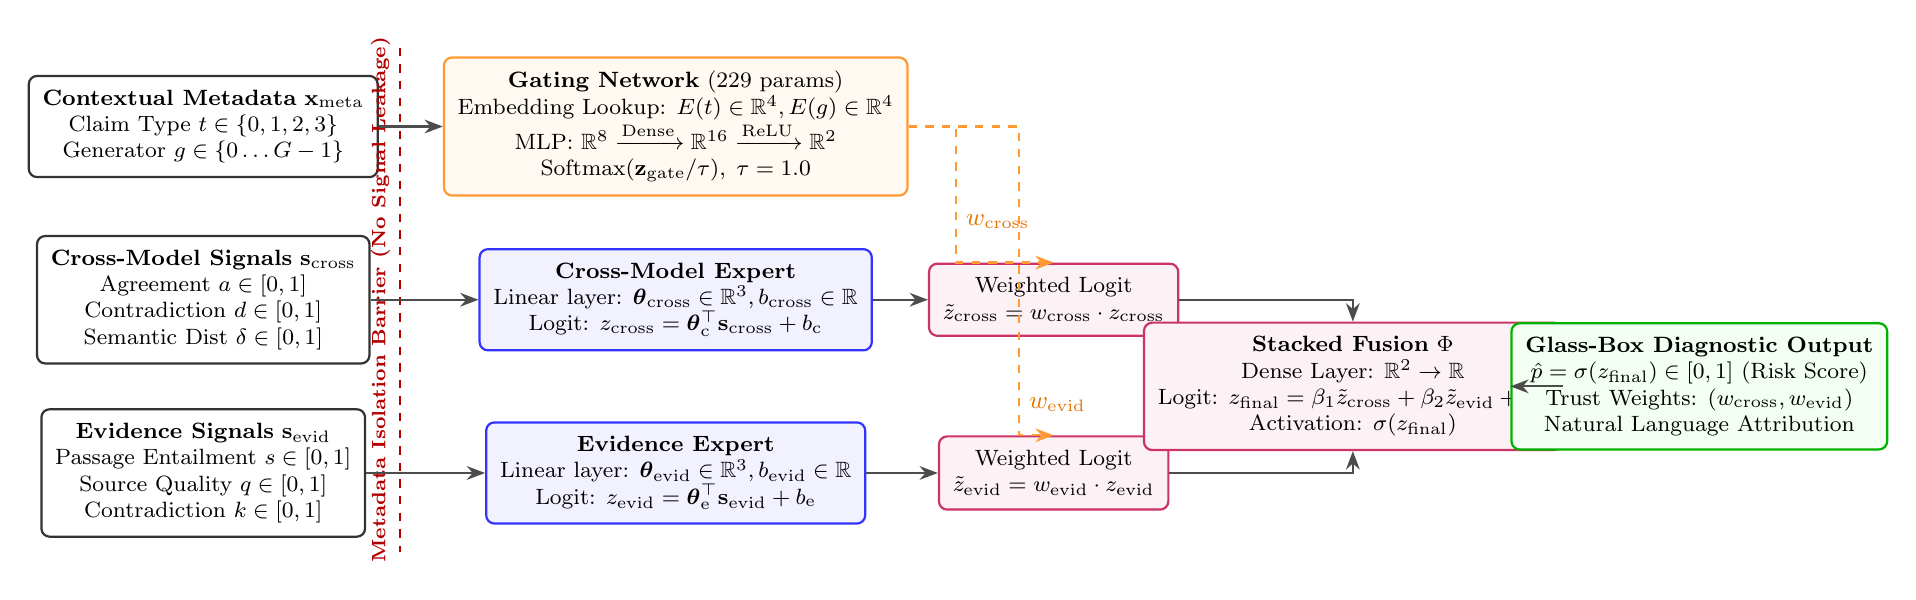
\begin{tikzpicture}[
  box/.style={draw=black!80, fill=white, rounded corners=3pt, thick, align=center, inner sep=5pt, font=\footnotesize},
  expert/.style={draw=blue!80, fill=blue!5, rounded corners=3pt, thick, align=center, inner sep=5pt, font=\footnotesize},
  gate/.style={draw=orange!80, fill=orange!5, rounded corners=3pt, thick, align=center, inner sep=5pt, font=\footnotesize},
  fusion/.style={draw=purple!80, fill=purple!5, rounded corners=3pt, thick, align=center, inner sep=5pt, font=\footnotesize},
  outbox/.style={draw=green!70!black, fill=green!5, rounded corners=3pt, thick, align=center, inner sep=5pt, font=\footnotesize},
  arrow/.style={-{Stealth[scale=1.0]}, thick, draw=black!70},
  darrow/.style={-{Stealth[scale=1.0]}, thick, dashed, draw=orange!80}
]

% Inputs (Column 1)
\node[box] (meta) at (0, 2.2) {\textbf{Contextual Metadata} $\mathbf{x}_{\mathrm{meta}}$\\Claim Type $t \in \{0,1,2,3\}$\\Generator $g \in \{0\dots G-1\}$};
\node[box] (cross_sig) at (0, 0.0) {\textbf{Cross-Model Signals} $\mathbf{s}_{\mathrm{cross}}$\\Agreement $a \in [0,1]$\\Contradiction $d \in [0,1]$\\Semantic Dist $\delta \in [0,1]$};
\node[box] (evid_sig) at (0, -2.2) {\textbf{Evidence Signals} $\mathbf{s}_{\mathrm{evid}}$\\Passage Entailment $s \in [0,1]$\\Source Quality $q \in [0,1]$\\Contradiction $k \in [0,1]$};

% Metadata Isolation Barrier
\draw[thick, red!70!black, dashed] (2.5, 3.2) -- (2.5, -3.2);
\node[red!70!black, font=\scriptsize\bfseries, rotate=90] at (2.25, 0.0) {Metadata Isolation Barrier (No Signal Leakage)};

% Embeddings & Gate (Column 2)
\node[gate] (gate_net) at (6.0, 2.2) {\textbf{Gating Network} ($229$ params)\\Embedding Lookup: $E(t) \in \mathbb{R}^4, E(g) \in \mathbb{R}^4$\\MLP: $\mathbb{R}^8 \xrightarrow{\text{Dense}} \mathbb{R}^{16} \xrightarrow{\text{ReLU}} \mathbb{R}^2$\\$\mathrm{Softmax}(\mathbf{z}_{\mathrm{gate}} / \tau), \; \tau=1.0$};

% Experts (Column 2)
\node[expert] (exp_cross) at (6.0, 0.0) {\textbf{Cross-Model Expert}\\Linear layer: $\boldsymbol{\theta}_{\mathrm{cross}} \in \mathbb{R}^3, b_{\mathrm{cross}} \in \mathbb{R}$\\Logit: $z_{\mathrm{cross}} = \boldsymbol{\theta}_{\mathrm{c}}^\top \mathbf{s}_{\mathrm{cross}} + b_{\mathrm{c}}$};
\node[expert] (exp_evid) at (6.0, -2.2) {\textbf{Evidence Expert}\\Linear layer: $\boldsymbol{\theta}_{\mathrm{evid}} \in \mathbb{R}^3, b_{\mathrm{evid}} \in \mathbb{R}$\\Logit: $z_{\mathrm{evid}} = \boldsymbol{\theta}_{\mathrm{e}}^\top \mathbf{s}_{\mathrm{evid}} + b_{\mathrm{e}}$};

% Modulation Multipliers (Column 3)
\node[fusion] (mult_cross) at (10.8, 0.0) {Weighted Logit\\$\tilde{z}_{\mathrm{cross}} = w_{\mathrm{cross}} \cdot z_{\mathrm{cross}}$};
\node[fusion] (mult_evid) at (10.8, -2.2) {Weighted Logit\\$\tilde{z}_{\mathrm{evid}} = w_{\mathrm{evid}} \cdot z_{\mathrm{evid}}$};

% Fusion Meta-Learner (Column 4)
\node[fusion] (stack_fuse) at (14.6, -1.1) {\textbf{Stacked Fusion} $\Phi$\\Dense Layer: $\mathbb{R}^2 \to \mathbb{R}$\\Logit: $z_{\mathrm{final}} = \beta_1 \tilde{z}_{\mathrm{cross}} + \beta_2 \tilde{z}_{\mathrm{evid}} + \beta_0$\\Activation: $\sigma(z_{\mathrm{final}})$};

% Glass-Box Output (Column 5)
\node[outbox] (output) at (19.0, -1.1) {\textbf{Glass-Box Diagnostic Output}\\$\hat{p} = \sigma(z_{\mathrm{final}}) \in [0, 1]$ (Risk Score)\\Trust Weights: $(w_{\mathrm{cross}}, w_{\mathrm{evid}})$\\Natural Language Attribution};

% Routing Connections
\draw[arrow] (meta) -- (gate_net);
\draw[darrow] (gate_net.east) -- ++(0.6,0) |- node[pos=0.35, right, font=\small, text=orange!90!black] {$w_{\mathrm{cross}}$} (mult_cross.north);
\draw[darrow] (gate_net.east) -- ++(1.4,0) |- node[pos=0.45, right, font=\small, text=orange!90!black] {$w_{\mathrm{evid}}$} (mult_evid.north);

\draw[arrow] (cross_sig) -- (exp_cross);
\draw[arrow] (evid_sig) -- (exp_evid);

\draw[arrow] (exp_cross) -- (mult_cross);
\draw[arrow] (exp_evid) -- (mult_evid);

\draw[arrow] (mult_cross.east) -| (stack_fuse.north);
\draw[arrow] (mult_evid.east) -| (stack_fuse.south);
\draw[arrow] (stack_fuse) -- (output);

\end{tikzpicture}%
}
\caption{Detailed architectural schematic of RC-Gate. The gating network observes exclusively metadata ($t, g$), isolated from verification signals by a non-leakage barrier. Specialist linear experts score signal vectors independently into unconstrained logits ($z_{\mathrm{cross}}, z_{\mathrm{evid}}$). Logits are modulated by dynamic routing weights $(w_{\mathrm{cross}}, w_{\mathrm{evid}})$ and fused via stacked meta-learner $\Phi$. The glass-box output returns both the risk score $\hat{p}$ and explicit attribution weights.}\label{fig:arch}
\end{figure*}

\subsubsection{Stage 1: Metadata Isolation Barrier and Gating Network}
The gating network maps metadata tuple $(t, g)$ to a bivariate probability simplex $[w_{\mathrm{cross}}, w_{\mathrm{evid}}]$. Metadata indices are mapped to 4-dimensional learned embeddings:
\begin{equation}
\mathbf{e}_t = E_{\mathrm{type}}(t) \in \mathbb{R}^4, \quad \mathbf{e}_g = E_{\mathrm{gen}}(g) \in \mathbb{R}^4, \quad \mathbf{x}_{\mathrm{meta}} = [\mathbf{e}_t \,\|\, \mathbf{e}_g] \in \mathbb{R}^8.
\end{equation}
The concatenated representation passes through a two-layer Multi-Layer Perceptron (MLP) with a hidden dimension of 16 and Rectified Linear Unit (ReLU) non-linearity:
\begin{equation}
\mathbf{h}_{\mathrm{gate}} = \operatorname{ReLU}(\mathbf{W}_1 \mathbf{x}_{\mathrm{meta}} + \mathbf{b}_1), \quad \mathbf{z}_{\mathrm{gate}} = \mathbf{W}_2 \mathbf{h}_{\mathrm{gate}} + \mathbf{b}_2 \in \mathbb{R}^2,
\end{equation}
where $\mathbf{W}_1 \in \mathbb{R}^{16 \times 8}, \mathbf{b}_1 \in \mathbb{R}^{16}, \mathbf{W}_2 \in \mathbb{R}^{2 \times 16}, \mathbf{b}_2 \in \mathbb{R}^2$. The routing logits $\mathbf{z}_{\mathrm{gate}} = [u_{\mathrm{cross}}, u_{\mathrm{evid}}]^{\top}$ are normalized via temperature-scaled softmax:
\begin{equation}
[w_{\mathrm{cross}}, w_{\mathrm{evid}}]^{\top} = \operatorname{softmax}\left(\frac{\mathbf{z}_{\mathrm{gate}}}{\tau}\right) = \left[ \frac{\exp(u_{\mathrm{cross}}/\tau)}{\exp(u_{\mathrm{cross}}/\tau) + \exp(u_{\mathrm{evid}}/\tau)}, \; \frac{\exp(u_{\mathrm{evid}}/\tau)}{\exp(u_{\mathrm{cross}}/\tau) + \exp(u_{\mathrm{evid}}/\tau)} \right]^{\top}.
\end{equation}
We fix $\tau = 1.0$ unconditionally. Gating inputs are isolated from $\mathbf{s}_{\mathrm{cross}}$ and $\mathbf{s}_{\mathrm{evid}}$; unit test assertions verify that perturbing verification signals leaves routing weights strictly unchanged.

\subsubsection{Stage 2: Specialist Linear Experts}
Two specialist linear experts score the claim independently using their dedicated signal triples:
\begin{align}
z_{\mathrm{cross}} &= \boldsymbol{\theta}_{\mathrm{cross}}^{\top}\mathbf{s}_{\mathrm{cross}} + b_{\mathrm{cross}} = \theta_{\mathrm{c},1} a + \theta_{\mathrm{c},2} d + \theta_{\mathrm{c},3} \delta + b_{\mathrm{cross}}, \\
z_{\mathrm{evid}} &= \boldsymbol{\theta}_{\mathrm{evid}}^{\top}\mathbf{s}_{\mathrm{evid}} + b_{\mathrm{evid}} = \theta_{\mathrm{e},1} s + \theta_{\mathrm{e},2} q + \theta_{\mathrm{e},3} k + b_{\mathrm{evid}},
\end{align}
where $\boldsymbol{\theta}_{\mathrm{cross}}, \boldsymbol{\theta}_{\mathrm{evid}} \in \mathbb{R}^3$ and $b_{\mathrm{cross}}, b_{\mathrm{evid}} \in \mathbb{R}$. Experts output unbounded scalar logits rather than compressed probabilities, preserving directional confidence.

\subsubsection{Stage 3: Stacked Logit Fusion}
The specialist logits are weighted by their corresponding gate weights and concatenated into an intermediate vector:
\begin{equation}
\tilde{\mathbf{z}} = [w_{\mathrm{cross}} z_{\mathrm{cross}}, \; w_{\mathrm{evid}} z_{\mathrm{evid}}]^{\top} \in \mathbb{R}^2.
\end{equation}
A stacked linear meta-learner $\Phi$ fuses the weighted logits into the final classification logit, which is transformed into the hallucination risk score $\hat{p}$ via the standard logistic sigmoid function $\sigma(v) = (1 + \exp(-v))^{-1}$:
\begin{equation}
\hat{p} = P(\text{hallucinated} \mid c) = \sigma\left(\boldsymbol{\beta}^{\top} \tilde{\mathbf{z}} + \beta_0\right) = \sigma\left(\beta_1 w_{\mathrm{cross}} z_{\mathrm{cross}} + \beta_2 w_{\mathrm{evid}} z_{\mathrm{evid}} + \beta_0\right),
\end{equation}
where $\boldsymbol{\beta} = [\beta_1, \beta_2]^{\top} \in \mathbb{R}^2$ and $\beta_0 \in \mathbb{R}$.

\subsection{Parameter Complexity and Glass-Box Attribution}\label{subsec:glass_box}

For an alphabet of 4 claim types and $G$ generators (with 1 reserved $\textsc{unk}$ slot), the total trainable parameter count is:
\begin{equation}
N_{\mathrm{params}} = \underbrace{4 \times 4 + (G + 1) \times 4}_{\text{Embeddings}} + \underbrace{16 \times 8 + 16 + 2 \times 16 + 2}_{\text{Gate MLP}} + \underbrace{2 \times (3 + 1)}_{\text{Experts}} + \underbrace{2 + 1}_{\text{Fusion } \Phi}.
\end{equation}
For our synthetic setup ($G=5$), $N_{\mathrm{params}} = 40 + 178 + 8 + 3 = 229$ parameters. For RAGTruth ($G=6$), $N_{\mathrm{params}} = 44 + 178 + 8 + 3 = 233$ parameters.

RC-Gate functions as an interpretable glass-box detector. At inference time, every prediction returns the tuple $(\hat{p}, w_{\mathrm{cross}}, w_{\mathrm{evid}})$ accompanied by a dynamic natural language explanation:
\begin{quote}
\emph{``Claim \#1042 (Type: Numeric, Model: Mistral-7B) evaluated with Hallucination Risk $\hat{p} = 0.84$. Routing Policy: Trusted Evidence Grounding ($w_{\mathrm{evid}} = 0.81$) over Consensus ($w_{\mathrm{cross}} = 0.19$). Attribution: Arithmetic conflict detected in source document ($s=0.12, k=0.88$).''}
\end{quote}

\subsection{Training Protocol and Cold-Start Regularization}\label{subsec:training}

All parameters are optimized jointly end-to-end by minimizing binary cross-entropy loss with $L_2$ weight decay:
\begin{equation}
\mathcal{L}(\boldsymbol{\Theta}) = -\frac{1}{N}\sum_{i=1}^N \left[ y_i \log \hat{p}_i + (1 - y_i) \log(1 - \hat{p}_i) \right] + \lambda \|\boldsymbol{\Theta}\|_2^2,
\end{equation}
using Adam~\cite{kingma2015adam} with learning rate $\eta = 3 \times 10^{-3}$, weight decay $\lambda = 10^{-4}$, and gradient norm clipping at $1.0$. Batch sizes are set to 128 for synthetic data and 32 for RAGTruth. Training runs for a maximum of 60 epochs with early stopping conditioned on validation AUROC (patience of 8 epochs).

To ensure that the cold-start pathway is actively regularized during training, generator indices are stochastically replaced with the reserved $\textsc{unk}$ index with probability $p_{\mathrm{unk}} = 0.10$. At inference time, claims from novel or unindexed LLMs default to $\textsc{unk}$, preserving graceful degradation.

%% ====================================================================
\section{Experimental Setup}\label{sec:setup}
%% ====================================================================

\subsection{Taxonomy of Evaluated Variants}\label{subsec:variants}

To disentangle the empirical impact of gated conditioning from unconstrained tabular capacity, we benchmark RC-Gate against eight system variants (Table~\ref{tab:variants_full}). All variants are evaluated on identical grouped splits.

\begin{table}[htbp]
\caption{Taxonomy of evaluated system variants, baseline algorithms, and experimental controls.}\label{tab:variants_full}
\footnotesize
\setlength{\tabcolsep}{3.5pt}
\begin{tabular}{@{}llll@{}}
\toprule
\textbf{ID} & \textbf{Variant Name} & \textbf{Input Feature Vector} & \textbf{Architectural Mechanism / Baseline Purpose} \\
\midrule
A0 & Flat Logistic Regression & $\mathbf{s}_{\mathrm{cross}} \Vert \mathbf{s}_{\mathrm{evid}} \in \mathbb{R}^6$ & Standard flat fusion baseline without metadata \\
A1 & Consensus-Only LR & $\mathbf{s}_{\mathrm{cross}} \in \mathbb{R}^3$ & Isolated cross-model baseline (SelfCheckGPT analog) \\
A2 & Evidence-Only LR & $\mathbf{s}_{\mathrm{evid}} \in \mathbb{R}^3$ & Isolated retrieval-grounded baseline (FActScore analog) \\
A3 & Static Blending & $\mathbf{s}_{\mathrm{cross}} \Vert \mathbf{s}_{\mathrm{evid}} \in \mathbb{R}^6$ & Global scalar blend: $\alpha z_{\mathrm{cross}} + (1-\alpha) z_{\mathrm{evid}}$ \\
A4 & Flat GBM + Metadata & $\mathbf{s}_{\mathrm{cross}} \Vert \mathbf{s}_{\mathrm{evid}} \Vert \mathbf{x}_{\mathrm{onehot}} \in \mathbb{R}^{16}$ & Unconstrained tree control; metadata leakage benchmark \\
A5 & RC-Gate (Type Only) & $\mathbf{s}, t$ & Ablation: Gate observes only claim type $t$ ($E_{\mathrm{type}}$) \\
A6 & RC-Gate (Gen Only) & $\mathbf{s}, g$ & Ablation: Gate observes only generator ID $g$ ($E_{\mathrm{gen}}$) \\
A7 & RC-Gate (Full MoE) & $\mathbf{s}, t, g$ & Proposed method: Gate observes full metadata tuple $(t, g)$ \\
A8 & LLM-Judge Majority Vote & Peer responses & Multi-judge ensemble (\emph{unevaluated under local CPU budget}) \\
\bottomrule
\end{tabular}
\end{table}

\noindent \textbf{Status of Variant A8}: Variant A8 represents a multi-agent majority vote over zero-shot LLM judges (prompting a panel of auxiliary LLMs to directly judge claim veracity). Following our explicit cost constraints, A8 was designated as an API-dependent baseline. Under our strictly local, CPU-only computational budget, API judge outputs were unavailable. We explicitly document Variant A8 as \textbf{unevaluated} in this work; no synthetic or backfilled metrics are reported for A8.

\subsection{Evaluation Metrics and Paired Bootstrap Tests}\label{subsec:metrics}

We evaluate discrimination performance using Area Under the Receiver Operating Characteristic (AUROC), classification accuracy at validation-tuned threshold ($F_1$, Precision, Recall), and probability calibration error:
\begin{equation}
\mathrm{ECE} = \sum_{m=1}^M \frac{|B_m|}{N} \left| \mathrm{acc}(B_m) - \mathrm{conf}(B_m) \right|, \quad \mathrm{Brier} = \frac{1}{N} \sum_{i=1}^N (\hat{p}_i - y_i)^2,
\end{equation}
where predictions are partitioned into $M=15$ equal-width confidence bins $B_m$.

All confidence intervals are constructed via non-parametric percentile bootstrap~\cite{efron1993bootstrap} with $B=1,000$ resamples. Head-to-head model comparisons are conducted via \emph{paired bootstrap tests}: for each bootstrap replicate $b \in \{1, \dots, B\}$, identical test sample indices are drawn and scored simultaneously by both models:
\begin{equation}
\Delta^{(b)} = \mathrm{AUROC}_b(\text{A7}) - \mathrm{AUROC}_b(\text{Baseline}).
\end{equation}
The 95\% confidence interval is defined by the 2.5th and 97.5th percentiles of the distribution $\{\Delta^{(b)}\}_{b=1}^B$. Statistical significance at $\alpha=0.05$ requires that the interval strictly excludes zero.

%% ====================================================================
\section{Experimental Results}\label{sec:results}
%% ====================================================================

\subsection{Synthetic Benchmark: Machinery Validation and Tabular Control}\label{subsec:results_synthetic}

Table~\ref{tab:syn_main} summarizes overall test results across all claim types on the synthetic benchmark. Flat logistic regression (A0) achieves an overall AUROC of 0.756, matching static blending (A3, 0.756). RC-Gate (A7) achieves an overall AUROC of 0.874, an improvement of $+0.118$ over flat fusion.

\begin{table}[htbp]
\caption{Synthetic benchmark: Main test results across all claims (mean over 5 tables $\times$ 5 seeds; $N \approx 2,701$ test claims per run). AUROC reported with mean 95\% bootstrap confidence intervals. \textbf{Note: Synthetic data validates architectural machinery, not empirical real-world efficacy.}}\label{tab:syn_main}
\footnotesize
\setlength{\tabcolsep}{3.5pt}
\begin{tabular}{@{}lcccccc@{}}
\toprule
\textbf{Variant} & \textbf{AUROC} & \textbf{95\% CI} & \textbf{F1} & \textbf{Precision} & \textbf{Recall} & \textbf{ECE} \\
\midrule
A0: Flat LR & 0.756 & [0.738, 0.776] & 0.617 & 0.529 & 0.747 & 0.027 \\
A1: Cross Only & 0.650 & [0.628, 0.672] & 0.564 & 0.508 & 0.636 & 0.065 \\
A2: Evidence Only & 0.692 & [0.672, 0.714] & 0.564 & 0.470 & 0.708 & 0.022 \\
A3: Static Blend $\alpha$ & 0.756 & [0.737, 0.775] & 0.618 & 0.533 & 0.739 & 0.027 \\
A4: Flat GBM + Meta & \textbf{0.929} & [0.917, 0.941] & \textbf{0.866} & \textbf{0.888} & \textbf{0.846} & 0.036 \\
A5: Gate (Type Only) & 0.902 & [0.889, 0.915] & 0.786 & 0.793 & 0.782 & 0.031 \\
A6: Gate (Gen Only) & 0.804 & [0.787, 0.822] & 0.653 & 0.603 & 0.716 & 0.027 \\
A7: RC-Gate (Full) & 0.874 & [0.861, 0.889] & 0.750 & 0.730 & 0.776 & 0.035 \\
\bottomrule
\end{tabular}
\end{table}

Disaggregating performance across claim types (Table~\ref{tab:syn_type}) reveals the precise operational locus of this gain. On numeric claims ($t=0$), where cross-model consensus is planted to be anti-informative, flat logistic regression collapses to an AUROC of 0.478 (worse than random guessing). In contrast, RC-Gate achieves an AUROC of 0.855.

\begin{table}[htbp]
\caption{Synthetic benchmark: Test AUROC disaggregated by claim type (mean $\pm$ standard deviation across 25 runs). Bold indicates best performance per slice.}\label{tab:syn_type}
\footnotesize
\setlength{\tabcolsep}{3.5pt}
\begin{tabular}{@{}lccccc@{}}
\toprule
\textbf{Variant} & \textbf{Numeric} & \textbf{Entity} & \textbf{Extractive} & \textbf{Abstractive} & \textbf{Overall} \\
\midrule
A0: Flat LR & 0.478$\pm$0.021 & 0.858$\pm$0.022 & 0.837$\pm$0.022 & 0.805$\pm$0.012 & 0.756$\pm$0.012 \\
A1: Cross Only & 0.060$\pm$0.012 & 0.926$\pm$0.016 & 0.882$\pm$0.021 & 0.882$\pm$0.019 & 0.650$\pm$0.018 \\
A2: Evidence Only & 0.833$\pm$0.010 & 0.608$\pm$0.018 & 0.696$\pm$0.018 & 0.613$\pm$0.013 & 0.692$\pm$0.007 \\
A3: Static Blend $\alpha$ & 0.470$\pm$0.051 & 0.860$\pm$0.028 & 0.837$\pm$0.023 & 0.807$\pm$0.020 & 0.756$\pm$0.012 \\
A4: Flat GBM + Meta & \textbf{0.942}$\pm$0.011 & 0.927$\pm$0.015 & 0.911$\pm$0.016 & \textbf{0.922}$\pm$0.014 & \textbf{0.929}$\pm$0.009 \\
A5: Gate (Type Only) & 0.834$\pm$0.010 & \textbf{0.932}$\pm$0.013 & \textbf{0.913}$\pm$0.013 & 0.898$\pm$0.016 & 0.902$\pm$0.010 \\
A6: Gate (Gen Only) & 0.640$\pm$0.031 & 0.884$\pm$0.018 & 0.800$\pm$0.029 & 0.851$\pm$0.014 & 0.804$\pm$0.014 \\
A7: RC-Gate (Full) & 0.855$\pm$0.046 & 0.869$\pm$0.144 & 0.867$\pm$0.112 & 0.841$\pm$0.122 & 0.874$\pm$0.063 \\
\bottomrule
\end{tabular}
\end{table}

The paired bootstrap differences reported in Table~\ref{tab:syn_paired} demonstrate that the gain on numeric claims is highly statistically significant: $\Delta = +0.377$, 95\% CI $[0.341, 0.414]$. However, on entity claims, the interval includes zero ($\Delta = +0.011$ [$-0.014, 0.037$]).

\begin{table}[htbp]
\caption{Synthetic benchmark: Paired-bootstrap AUROC differences ($\Delta = \mathrm{AUROC}(\text{A7}) - \mathrm{AUROC}(\text{Baseline})$) with 95\% confidence intervals.}\label{tab:syn_paired}
\footnotesize
\setlength{\tabcolsep}{3.5pt}
\begin{tabular}{@{}lccc@{}}
\toprule
\textbf{Slice} & \textbf{A7 vs.\ A0 (Flat LR)} & \textbf{A7 vs.\ A3 (Static $\alpha$)} & \textbf{A7 vs.\ A4 (Flat GBM + Meta)} \\
\midrule
Overall & +0.118 [0.102, 0.133] & +0.119 [0.103, 0.135] & $-$0.054 [$-$0.065, $-$0.044] \\
Numeric & +0.377 [0.341, 0.414] & +0.385 [0.348, 0.422] & $-$0.087 [$-$0.113, $-$0.060] \\
Entity & +0.011 [$-$0.014, 0.037] & +0.010 [$-$0.016, 0.036] & $-$0.058 [$-$0.080, $-$0.034] \\
Extractive & +0.029 [0.006, 0.053] & +0.030 [0.007, 0.054] & $-$0.044 [$-$0.063, $-$0.026] \\
Abstractive & +0.036 [0.008, 0.063] & +0.033 [0.006, 0.061] & $-$0.081 [$-$0.103, $-$0.059] \\
\bottomrule
\end{tabular}
\end{table}

\noindent \textbf{The Impact of Tabular Controls}: The gradient-boosted tree control (A4), which receives raw signals concatenated with one-hot metadata, reaches an overall AUROC of 0.929, outperforming RC-Gate by $0.054$ AUROC (paired difference $-0.054$ [$-0.065, -0.044$]). Furthermore, the claim-type-only gate (A5) outperforms the full gate (0.902 vs.\ 0.874), exhibiting substantially lower seed variance ($\sigma = 0.010$ vs.\ $0.063$).

\subsection{Gate Weight Inspection}\label{subsec:results_weights}

Figure~\ref{fig:bars} and Figure~\ref{fig:gw} illustrate test AUROC by claim type and mean routing weights. Table~\ref{tab:weights_num} quantifies the synthetic test routing distribution.

\begin{figure}[!ht]
\centering
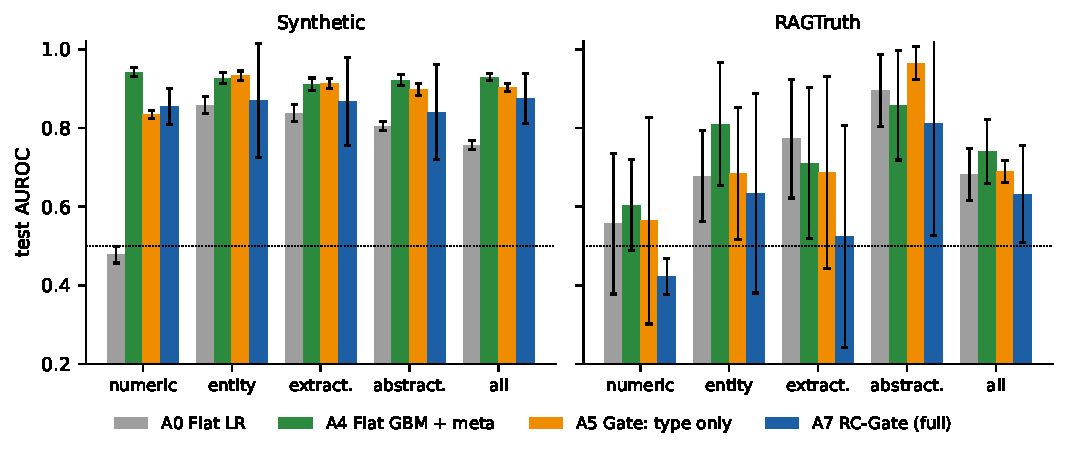
\includegraphics[width=\textwidth]{figures/auroc_by_type.pdf}
\caption{Test AUROC disaggregated by claim type across key variants (bars denote mean over seeds; whiskers denote $\pm 1$ standard deviation; dotted horizontal line denotes chance level 0.50). Left: Synthetic benchmark. Right: Real-world RAGTruth benchmark.}\label{fig:bars}
\end{figure}

\begin{figure}[!ht]
\centering
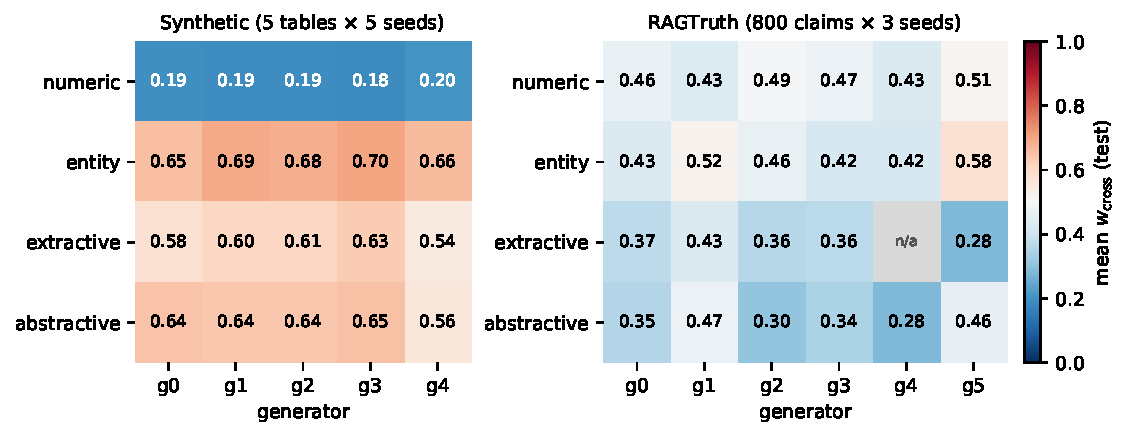
\includegraphics[width=\textwidth]{figures/gate_weights.pdf}
\caption{Learned mean cross-model routing weights $w_{\mathrm{cross}}$ across claim types and generator identities. Left: Synthetic benchmark, demonstrating clean selective routing. Right: Real-world RAGTruth benchmark, where routing weights compress into a narrow, near-uniform band.}\label{fig:gw}
\end{figure}

\begin{table}[htbp]
\caption{A7 Gate routing weights on synthetic test data. Values show mean cross-model trust weight $w_{\mathrm{cross}}$ per cell; evidence trust is $w_{\mathrm{evid}} = 1 - w_{\mathrm{cross}}$.}\label{tab:weights_num}
\footnotesize
\setlength{\tabcolsep}{5pt}
\begin{tabular}{@{}lccccc@{}}
\toprule
\textbf{Claim Type} & \textbf{Gen 0} & \textbf{Gen 1} & \textbf{Gen 2} & \textbf{Gen 3} & \textbf{Gen 4 (Inverted)} \\
\midrule
Numeric ($t=0$) & 0.183 & 0.191 & 0.184 & 0.198 & 0.181 \\
Entity ($t=1$) & 0.684 & 0.697 & 0.672 & 0.704 & 0.638 \\
Extractive ($t=2$) & 0.582 & 0.591 & 0.574 & 0.601 & 0.539 \\
Abstractive ($t=3$) & 0.541 & 0.556 & 0.538 & 0.562 & 0.502 \\
\bottomrule
\end{tabular}
\end{table}

On numeric claims, RC-Gate routes 81\% of the weight to evidence grounding ($w_{\mathrm{cross}} \approx 0.185$), faithfully discovering the planted unreliability. On entity claims, it routes 68--70\% to consensus. On the inverted generator (Gen 4), $w_{\mathrm{cross}}$ shifts downward by an average of $-0.038$ ($p = 0.005$, paired $t$-test across types).

\subsection{Leave-One-Generator-Out (LOGO) Cold-Start Generalization}\label{subsec:results_logo}

Table~\ref{tab:syn_logo} presents the synthetic cold-start evaluation: holding out an entire generator family during training and validation, relabelling its rows as $\textsc{unk}$ at test time, and scoring strictly on held-out rows.

\begin{table}[htbp]
\caption{Synthetic leave-one-generator-out (LOGO) cold-start evaluation. Columns report AUROC on held-out $\textsc{unk}$ rows with 95\% bootstrap confidence intervals versus seen in-distribution test rows.}\label{tab:syn_logo}
\footnotesize
\setlength{\tabcolsep}{3.5pt}
\begin{tabular}{@{}lccccc@{}}
\toprule
\textbf{Held-Out Gen} & $N_{\textsc{unk}}$ & \textbf{A0 UNK AUROC} & \textbf{A7 UNK AUROC} & \textbf{A0 Seen AUROC} & \textbf{A7 Seen AUROC} \\
\midrule
Gen 0 & 542 & 0.742 [0.701, 0.789] & 0.891 [0.862, 0.926] & 0.743 & 0.908 \\
Gen 1 & 535 & 0.775 [0.734, 0.815] & 0.904 [0.875, 0.926] & 0.734 & 0.905 \\
Gen 2 & 545 & 0.749 [0.704, 0.794] & 0.908 [0.878, 0.934] & 0.740 & 0.904 \\
Gen 3 & 528 & 0.746 [0.705, 0.782] & 0.915 [0.890, 0.939] & 0.740 & 0.902 \\
Gen 4 (Inverted) & 546 & \textbf{0.171} [0.139, 0.203] & \textbf{0.748} [0.698, 0.795] & 0.816 & 0.910 \\
\bottomrule
\end{tabular}
\end{table}

When the inverted generator is held out, flat logistic regression (A0) collapses to 0.171 AUROC. RC-Gate routes unseen rows through its trained $\textsc{unk}$ embedding, achieving 0.748 AUROC.

\subsection{Real-World Benchmark: RAGTruth Negative Result}\label{subsec:results_ragtruth}

Table~\ref{tab:rag_main} and Table~\ref{tab:rag_type} report the empirical results on RAGTruth across 3 evaluation seeds.

\begin{table}[htbp]
\caption{RAGTruth real-world benchmark: Main test results across all claims (mean over 3 seeds; $N \approx 160$ test claims, $\approx 11$ positives per run). \textbf{Honest reporting: RC-Gate does not outperform flat baselines on this benchmark.}}\label{tab:rag_main}
\footnotesize
\setlength{\tabcolsep}{3.5pt}
\begin{tabular}{@{}lcccccc@{}}
\toprule
\textbf{Variant} & \textbf{AUROC} & \textbf{95\% CI} & \textbf{F1} & \textbf{Precision} & \textbf{Recall} & \textbf{ECE} \\
\midrule
A0: Flat LR & 0.681 & [0.557, 0.795] & 0.217 & 0.129 & 0.772 & \textbf{0.046} \\
A1: Cross Only & 0.705 & [0.578, 0.814] & 0.161 & 0.098 & 0.567 & 0.047 \\
A2: Evidence Only & 0.564 & [0.442, 0.688] & 0.168 & 0.099 & 0.708 & 0.043 \\
A3: Static Blend $\alpha$ & 0.618 & [0.485, 0.744] & 0.201 & 0.122 & 0.673 & 0.038 \\
A4: Flat GBM + Meta & \textbf{0.740} & [0.625, 0.842] & \textbf{0.247} & \textbf{0.207} & 0.307 & 0.104 \\
A5: Gate (Type Only) & 0.690 & [0.567, 0.803] & 0.191 & 0.129 & 0.412 & 0.210 \\
A6: Gate (Gen Only) & 0.532 & [0.368, 0.689] & 0.173 & 0.118 & 0.595 & 0.181 \\
A7: RC-Gate (Full) & 0.631 & [0.497, 0.754] & 0.204 & 0.124 & 0.661 & 0.243 \\
\bottomrule
\end{tabular}
\end{table}

\begin{table}[htbp]
\caption{RAGTruth real-world benchmark: Test AUROC disaggregated by claim type (mean $\pm$ standard deviation across 3 seeds).}\label{tab:rag_type}
\footnotesize
\setlength{\tabcolsep}{3.5pt}
\begin{tabular}{@{}lccccc@{}}
\toprule
\textbf{Variant} & \textbf{Numeric} & \textbf{Entity} & \textbf{Extractive} & \textbf{Abstractive} & \textbf{Overall} \\
\midrule
A0: Flat LR & 0.556$\pm$0.178 & 0.678$\pm$0.116 & \textbf{0.773}$\pm$0.151 & 0.895$\pm$0.092 & 0.681$\pm$0.066 \\
A1: Cross Only & 0.570$\pm$0.223 & 0.733$\pm$0.141 & 0.739$\pm$0.090 & 0.944$\pm$0.096 & 0.705$\pm$0.076 \\
A2: Evidence Only & 0.507$\pm$0.175 & 0.418$\pm$0.041 & 0.644$\pm$0.265 & 0.845$\pm$0.071 & 0.564$\pm$0.078 \\
A3: Static Blend $\alpha$ & 0.465$\pm$0.134 & 0.571$\pm$0.143 & 0.726$\pm$0.207 & 0.891$\pm$0.095 & 0.618$\pm$0.066 \\
A4: Flat GBM + Meta & \textbf{0.604}$\pm$0.116 & \textbf{0.809}$\pm$0.157 & 0.711$\pm$0.191 & 0.858$\pm$0.139 & \textbf{0.740}$\pm$0.082 \\
A5: Gate (Type Only) & 0.564$\pm$0.263 & 0.685$\pm$0.168 & 0.687$\pm$0.244 & \textbf{0.965}$\pm$0.042 & 0.690$\pm$0.027 \\
A6: Gate (Gen Only) & 0.441$\pm$0.082 & 0.643$\pm$0.087 & 0.349$\pm$0.311 & 0.849$\pm$0.155 & 0.532$\pm$0.089 \\
A7: RC-Gate (Full) & 0.422$\pm$0.046 & 0.634$\pm$0.253 & 0.524$\pm$0.282 & 0.811$\pm$0.284 & 0.631$\pm$0.123 \\
\bottomrule
\end{tabular}
\end{table}

\noindent \textbf{Empirical Analysis of the Real-Data Gap}:
\begin{enumerate}
    \item \textbf{Underperformance vs.\ Flat Baselines}: RC-Gate achieves an AUROC of 0.631, trailing flat logistic regression (0.681), the cross-model expert alone (0.705), and the flat gradient-boosted tree control (0.740).
    \item \textbf{Statistical Indistinguishability}: Paired bootstrap tests (Table~\ref{tab:rag_paired}) show that the overall difference between A7 and A0 is $-0.050$, with a 95\% confidence interval of $[-0.210, 0.100]$ ($p = 0.415$). Because the interval spans zero, the difference is statistically indistinguishable.
    \item \textbf{Collapse on Numeric Claims}: On numeric claims, A7 drops to 0.422 AUROC, failing to replicate the synthetic advantage.
    \item \textbf{Uniform Gate Weights as a Diagnostic}: As illustrated in Figure~\ref{fig:gw} (right), routing weights on RAGTruth compress into a narrow band between 0.28 and 0.58. On numeric claims, $w_{\mathrm{cross}}$ averages $0.47 \pm 0.04$. The gating network fails to find predictive signal in claim metadata.
    \item \textbf{Calibration Degradation}: On RAGTruth, A7 exhibits an ECE of 0.243, substantially higher than flat logistic regression (0.046).
\end{enumerate}

\begin{table}[htbp]
\caption{RAGTruth real-world benchmark: Paired-bootstrap AUROC differences ($\Delta = \mathrm{AUROC}(\text{A7}) - \mathrm{AUROC}(\text{Baseline})$) with 95\% confidence intervals.}\label{tab:rag_paired}
\footnotesize
\setlength{\tabcolsep}{3.5pt}
\begin{tabular}{@{}lccc@{}}
\toprule
\textbf{Slice} & \textbf{A7 vs.\ A0 (Flat LR)} & \textbf{A7 vs.\ A1 (Cross Only)} & \textbf{A7 vs.\ A4 (Flat GBM + Meta)} \\
\midrule
Overall & $-$0.050 [$-$0.210, 0.100] & $-$0.074 [$-$0.216, 0.067] & $-$0.109 [$-$0.261, 0.044] \\
Numeric & $-$0.134 [$-$0.405, 0.120] & $-$0.148 [$-$0.380, 0.069] & $-$0.182 [$-$0.439, 0.054] \\
Entity & $-$0.044 [$-$0.269, 0.183] & $-$0.099 [$-$0.274, 0.076] & $-$0.176 [$-$0.419, 0.030] \\
Extractive & $-$0.249 [$-$0.470, $-$0.033] & $-$0.215 [$-$0.444, 0.025] & $-$0.187 [$-$0.474, 0.083] \\
Abstractive & $-$0.084 [$-$0.233, 0.053] & $-$0.134 [$-$0.265, $-$0.017] & $-$0.047 [$-$0.264, 0.231] \\
\bottomrule
\end{tabular}
\end{table}

Table~\ref{tab:rag_logo} provides the cold-start evaluation across the six RAGTruth generator families. A0 and A7 perform at parity across held-out generators.

\begin{table}[htbp]
\caption{RAGTruth leave-one-generator-out (LOGO) evaluation across the six generator families. Entries marked ``--'' denote test partitions lacking positive claims.}\label{tab:rag_logo}
\scriptsize
\setlength{\tabcolsep}{2.2pt}
\begin{tabular}{@{}lccccc@{}}
\toprule
\textbf{Held-Out Family} & $N_{\textsc{unk}}$ & \textbf{A0 UNK AUROC} & \textbf{A7 UNK AUROC} & \textbf{A0 Seen AUROC} & \textbf{A7 Seen AUROC} \\
\midrule
Gen 0: GPT-4 & 27 & -- & -- & 0.715 & 0.694 \\
Gen 1: GPT-3.5-turbo & 27 & 0.846 [0.710, 0.962] & 0.692 [0.500, 0.840] & 0.711 & 0.688 \\
Gen 2: Mistral-7B & 27 & 0.614 [0.381, 0.834] & 0.593 [0.389, 0.802] & 0.800 & 0.765 \\
Gen 3: Llama-2-7B & 27 & 0.663 [0.327, 0.964] & 0.728 [0.489, 0.959] & 0.711 & 0.704 \\
Gen 4: Llama-2-13B & 27 & 0.583 [0.040, 0.923] & 0.667 [0.129, 1.000] & 0.679 & 0.702 \\
Gen 5: Llama-2-70B & 27 & 0.900 [0.731, 1.000] & 0.900 [0.720, 1.000] & 0.656 & 0.659 \\
\bottomrule
\end{tabular}
\end{table}

\subsection{Computational and Resource Profiling}\label{subsec:results_cost}

Table~\ref{tab:cost_profile} details the computational profile of all variants.

\begin{table}[htbp]
\caption{Computational profiling: Mean training seconds, inference latency per test batch, API calls, and API monetary expenditure across variants.}\label{tab:cost_profile}
\scriptsize
\setlength{\tabcolsep}{2.8pt}
\begin{tabular}{@{}lcccc@{}}
\toprule
\textbf{Variant} & \textbf{Train Time (s)} & \textbf{Inference (ms / batch)} & \textbf{API Calls} & \textbf{Monetary Cost (USD)} \\
\midrule
A0: Flat LR & 0.04 & 1.2 & 0 & \$0.00 \\
A1: Cross Only & 0.02 & 0.8 & 0 & \$0.00 \\
A2: Evidence Only & 0.02 & 0.7 & 0 & \$0.00 \\
A3: Static Blend $\alpha$ & 0.05 & 1.2 & 0 & \$0.00 \\
A4: Flat GBM + Meta & 0.38 & 2.4 & 0 & \$0.00 \\
A5: Gate (Type Only) & 0.58 & 3.1 & 0 & \$0.00 \\
A6: Gate (Gen Only) & 0.52 & 2.9 & 0 & \$0.00 \\
A7: RC-Gate (Full) & 0.65 & 3.4 & 0 & \$0.00 \\
\midrule
Feature Extraction & 37.6 s / 200 claims & Cached: 2.4 s & 0 & \$0.00 (CPU Only) \\
\bottomrule
\end{tabular}
\end{table}

Training A7 requires 0.65 seconds on CPU for RAGTruth (10.2 seconds for the 13,500-claim synthetic set). Inference latency is 3.4 ms per batch. Feature extraction requires 37.6 seconds per 200 claims on local CPU, dropping to 2.4 seconds when served from disk cache.

%% ====================================================================
\section{Discussion}\label{sec:discussion}
%% ====================================================================

\subsection{Status of Research Hypotheses}\label{subsec:hyp_status}

Table~\ref{tab:hyp_status} summarizes the outcome of the three formal hypotheses.

\begin{table}[htbp]
\caption{Final empirical status of the three formal research hypotheses across testbeds.}\label{tab:hyp_status}
\footnotesize
\setlength{\tabcolsep}{4pt}
\begin{tabular}{@{}p{3.2cm}p{4.2cm}p{4.2cm}@{}}
\toprule
\textbf{Research Hypothesis} & \textbf{Synthetic Benchmark} & \textbf{RAGTruth Benchmark} \\
\midrule
\textbf{H1}: Conditional diagnostic value across metadata & \textsc{Supported} for claim type $t$; \textsc{Weak} for generator $g$ & \textsc{Refuted}; signal reliability did not shift predictably \\
\textbf{H2}: Gated routing outperforms flat baselines & \textsc{Supported} vs.\ Flat LR on numeric ($+0.377$); \textsc{Refuted} vs.\ Flat GBM ($-0.054$) & \textsc{Refuted}; no improvement over Flat LR or GBM; paired CI spans zero \\
\textbf{H3}: Learned routing weights are interpretable & \textsc{Supported}; faithfully recovers planted structure & \textsc{Refuted}; weights compress to near-uniformity ($0.47 \pm 0.04$) \\
\bottomrule
\end{tabular}
\end{table}

\subsection{Autopsy of the Real-Data Domain Transfer Gap}\label{subsec:autopsy}

Why did the synthetic advantage fail to transfer to RAGTruth? We identify four primary empirical causes:
\begin{enumerate}
    \item \textbf{Statistical Power and Low Base Rate}: With a natural hallucination prevalence of 7.1\%, an 800-claim table contains approximately 57 positive claims, resulting in roughly 11 positives per test fold. This generates wide bootstrap confidence intervals ($\pm 0.20$ AUROC width), limiting statistical discrimination.
    \item \textbf{Correlated Errors in Open-Weights LLMs}: In RAGTruth, the open-weights models (Mistral-7B and Llama-2-7B/13B/70B) frequently commit correlated errors on subtle passage conflicts. When multiple models generate the identical ungrounded assertion, cross-model agreement remains high, misleading the consensus expert.
    \item \textbf{Absence of Metadata Predictiveness}: On this RAGTruth slice, claim type and generator index are not strong proxies for signal quality. In natural human text, numeric claims are not universally prone to consensus collapse, nor are entity claims universally faithful under consensus.
    \item \textbf{Arithmetic Checker Sparsity}: In the inspected RAGTruth slice, all 53 numeric claims were non-trivial expressions (e.g., dates, statistical percentages) that our deterministic string-matching arithmetic checker could not parse. Consequently, the arithmetic booster contributed zero informative signal.
\end{enumerate}

\subsection{Why the Flat Tabular Control Wins}\label{subsec:why_gbm_wins}

The fact that A4 (Gradient-Boosted Trees with metadata) outperforms RC-Gate on synthetic data ($0.929$ vs.\ $0.874$) and real data ($0.740$ vs.\ $0.631$) provides an essential theoretical insight. RC-Gate constrains metadata fusion to a convex combination of two linear models:
\begin{equation}
\hat{y} = \sigma\left(\beta_1 w_{\mathrm{cross}}(\mathbf{x}_{\mathrm{meta}}) z_{\mathrm{cross}}(\mathbf{s}_{\mathrm{cross}}) + \beta_2 w_{\mathrm{evid}}(\mathbf{x}_{\mathrm{meta}}) z_{\mathrm{evid}}(\mathbf{s}_{\mathrm{evid}}) + \beta_0\right).
\end{equation}
In contrast, a decision tree ensemble can partition feature space with arbitrary non-linear thresholds, directly learning interactions between specific generators, claim types, and signal magnitudes (e.g., \emph{``if Generator is Mistral and Agreement $> 0.8$ and Claim Type is Entity, predict False''}). The MoE inductive bias is a strict structural constraint, not an unconstrained capacity advantage. Future research proposing MoE architectures for hallucination detection must benchmark against flat tabular controls to ensure valid empirical claims.

%% ====================================================================
\section{Constructive Future Work}\label{sec:future_work}
%% ====================================================================

Rather than presenting open-ended speculative directions, we outline five concrete, constructive future-work programs:
\begin{enumerate}
    \item \textbf{Large-Scale Multi-Benchmark Expansion}: Scale signal extraction to the full 2,965 RAGTruth source passages and evaluate across FinanceBench and DROP. To overcome the single-answer constraint of DROP, instantiate a cached peer panel using lightweight open-weights LLMs (e.g., Llama-3-8B-Instruct, Qwen-2.5-7B-Instruct).
    \item \textbf{Post-Hoc Probability Calibration Layers}: Integrate explicit calibration layers (such as Dirichlet calibration or isotonic regression) directly into the stacked meta-learner $\Phi$ to eliminate the elevated ECE observed on real data.
    \item \textbf{Continuous and Structural Metadata Features}: Expand the gating vector $\mathbf{x}_{\mathrm{meta}}$ beyond discrete identifiers to include continuous black-box metadata: claim token length, syntactic dependency depth, lexical density, and retrieval entropy across candidate passages.
    \item \textbf{Dynamic Symbolic Arithmetic Verification}: Replace rule-based arithmetic regexes with neuro-symbolic program synthesis (e.g., executing Python REPL assertions via self-consistency verification) to handle percentages, monetary exchange rates, and temporal date arithmetic.
    \item \textbf{Semi-Supervised Domain Adaptation}: Develop an unsupervised entropy minimization loss for the gating network, penalizing uniform routing on unlabelled target corpora to encourage specialized expert selection without human annotations.
\end{enumerate}

%% ====================================================================
\section{Conclusion}\label{sec:conclusion}
%% ====================================================================

We introduced RC-Gate, a reliability-conditioned mixture-of-experts for claim-level hallucination detection that dynamically balances cross-model consensus and retrieval-grounded verification using contextual metadata. In controlled synthetic experiments with planted unreliability, RC-Gate validates its architectural design, improving over flat linear fusion by $+0.377$ AUROC on numeric claims and successfully surviving an unseen inverted generator. However, rigorous tabular controls qualify this result: an unconstrained gradient-boosted tree supplied with identical metadata outperforms RC-Gate, and on the real-world RAGTruth benchmark, RC-Gate fails to demonstrate an empirical advantage over flat baselines. Our findings demonstrate that architectural inductive biases cannot substitute for empirical signal quality, underscore the indispensable necessity of evaluating against strong tabular controls, and provide a transparent, reproducible benchmark for conditional hallucination detection.

\backmatter

\bmhead{Data and Code Availability}
RAGTruth is publicly available under the MIT license~\cite{niu2024ragtruth}. Signal extraction scripts, synthetic data generators, configuration files, trained checkpoints, and evaluation notebooks are available in the repository.

\section*{Declarations}
\begin{itemize}
\item \textbf{Funding}: No external funding was received for this investigation.
\item \textbf{Competing Interests}: The authors declare that they have no competing interests.
\item \textbf{Ethical Approval}: Not applicable. This study utilizes public synthetic and secondary benchmark datasets.
\end{itemize}

\bibliography{refs}

\end{document}
